\pdfminorversion=7
\PassOptionsToPackage{obeyspaces}{url}
\documentclass[latin1, english, usepdftitle=false, svgnames, color="table, fixpdftex, hyperref, fixinclude, xcdraw", t]{beamer}


\usepackage{latexscholar-i18n}
\usepackage{latexscholar-verbatim}
\usepackage{lode-imacid}
\usepackage{latexscholar-pdf}

\usepackage{animate}

\usepackage{inputx}
\inputpaths{../CommonAssets/}

\graphicspath{{../CommonAssets/}}


\title{Software testing}
\subtitle{Structural testing}
\author[]{%
	Marco Aur�lio Graciotto Silva\inst{1}, \and
	Ellen Francine Barbosa\inst{2}, \\\and
	M�rcio Eduardo Delamaro\inst{2}, \and
	Auri Marcelo Rizzo Vincenzi\inst{3}, \\\and
	Jos� Carlos Maldonado\inst{2}
}

\newcommand{\numberofinstitutes}{3}
\institute[ICMC]
{
	\inst{1}%
%	\textbf{Department of Computing}\\
	Federal University of Technology -- Paran� (UTFPR)\\
	Campo Mour�o, PR, Brazil
	\and
	\inst{2}%
%	\textbf{Institute of Mathematical Sciences and Computing}\\
	University of S�o Paulo (USP)\\
	S�o Carlos, SP, Brazil
	\and
	\inst{3}
%	\textbf{Department of Computing}\\
	Federal University of S�o Carlos (UFSCar)\\
	S�o Carlos, SP, Brazil
}

\date[]{2017}
\logopicture{figs/icmc-qualipso-inf}

\begin{document}

\frontmatter{}
\begin{frame}[c, plain]
\label{title}
\titlepage
\end{frame}

%\begin{frame}[c,parent={title}, hasprev=false, hasnext=false]
%\frametitle{Software Testing}
%\label{cmap:software-testing}
%
%\insertcmap{Courses-SoftwareTesting-SoftwareTesting}
%\end{frame}

\begin{frame}[c,parent={title}, hasprev=false, hasnext=false]
\frametitle{Software Testing}
\label{cmap:software-testing}

\centering
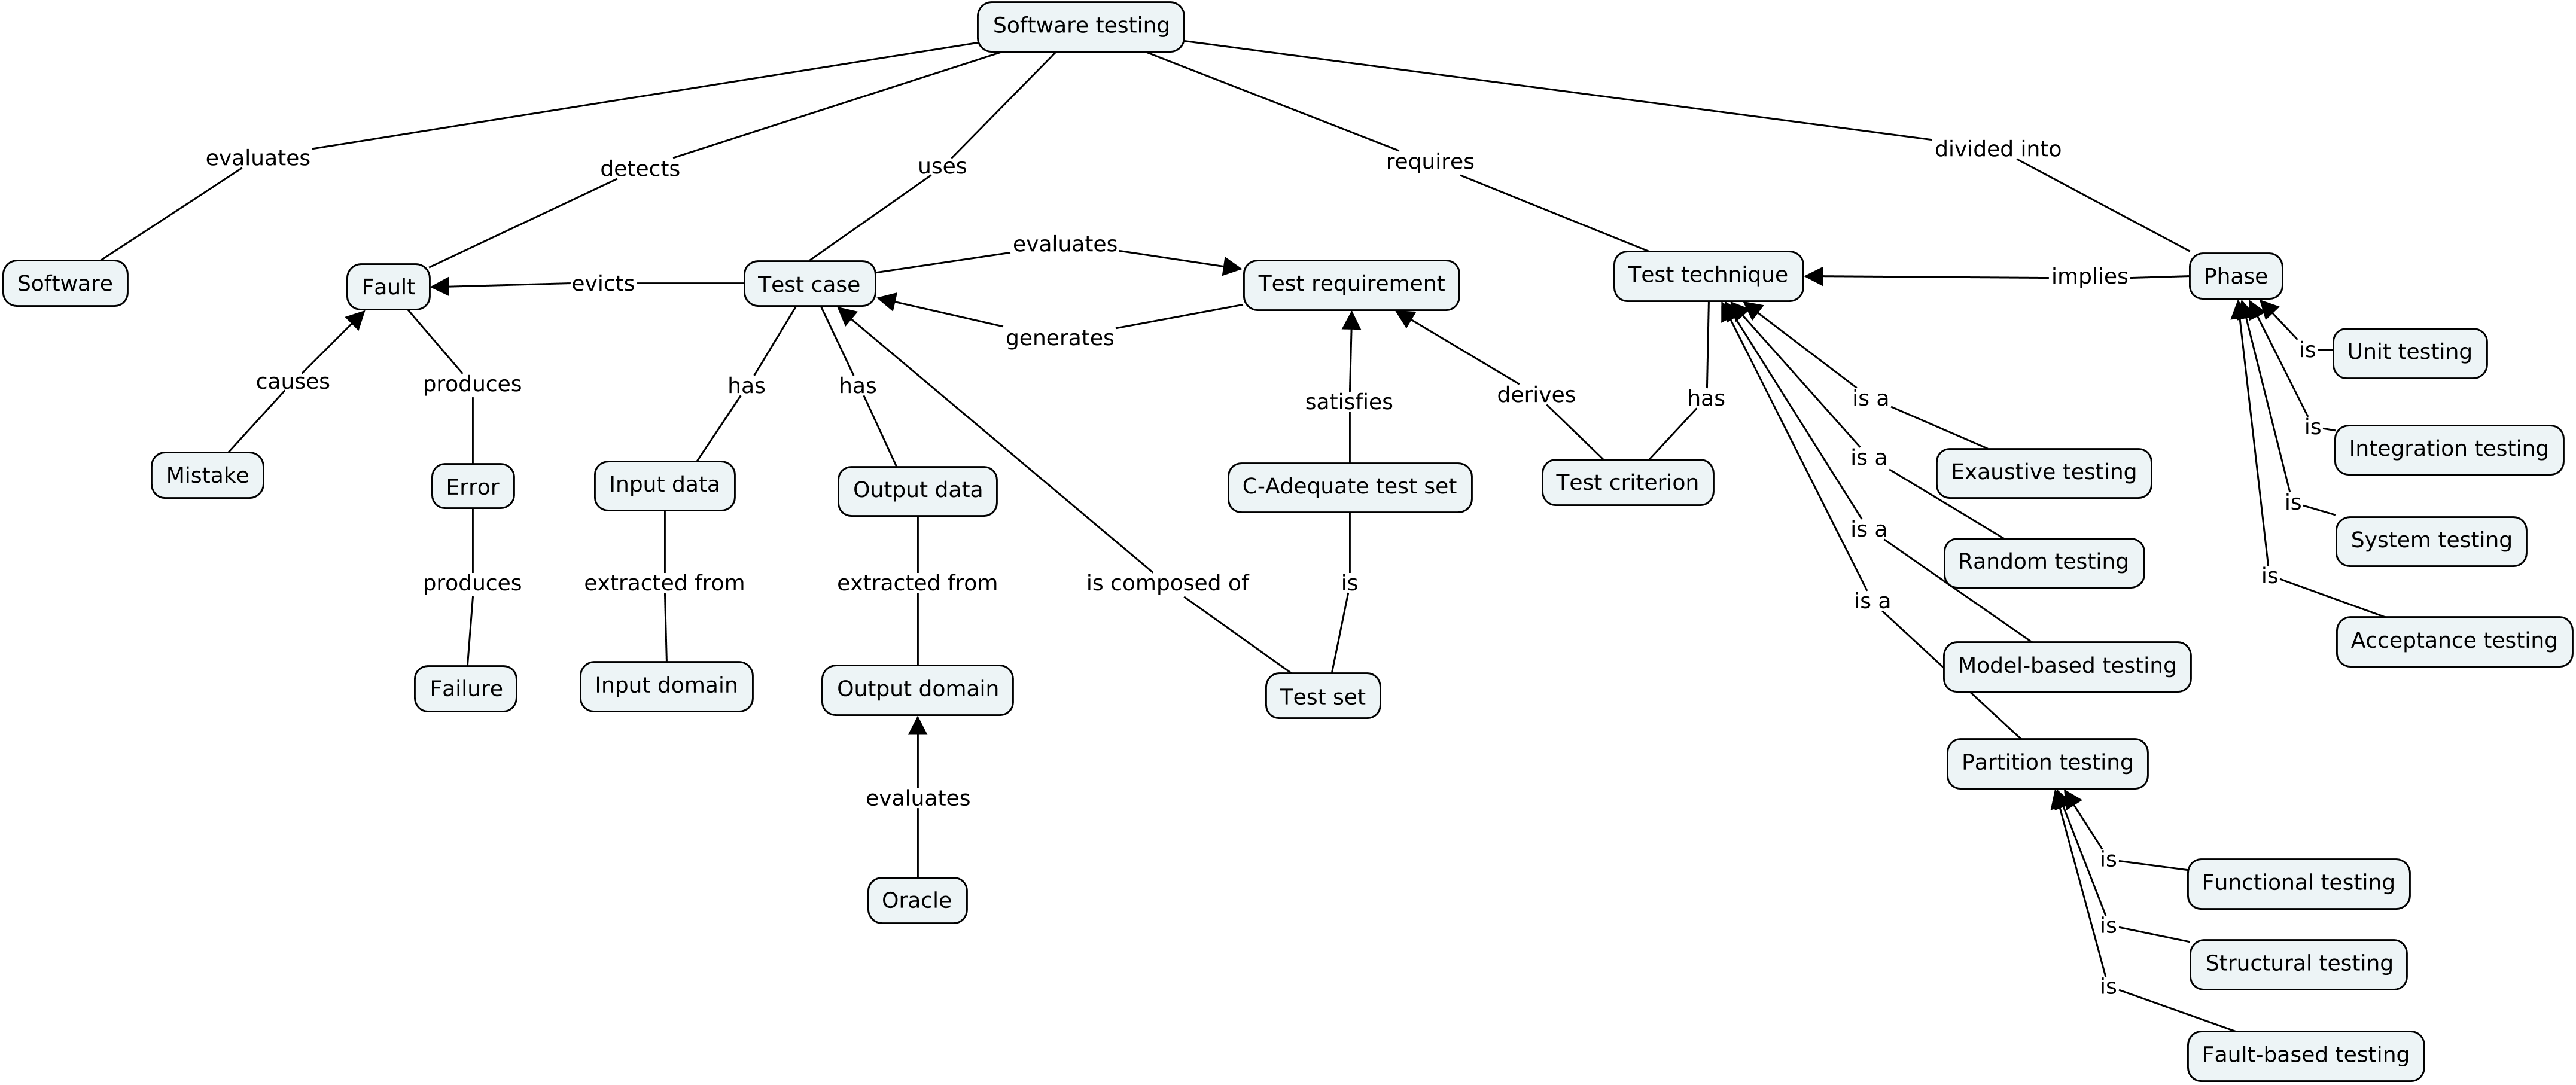
\includegraphics[width=\textwidth]{../BasicConcepts/Software testing fundamentals.png}
\end{frame}


\mainmatter{}

% Structural software testing module
%
\part{Structural software Testing}
\section{Structural software testing}
\begin{frame}[parent={cmap:software-testing}, hasprev=false, hasnext=true]
\frametitle{Structural testing}
\label{cmap:structural-software-testing}
\label{cmap:structural-testing}

\insertcmap{Courses-SoftwareTesting-StructuralTesting}
\end{frame}



\begin{frame}[parent={cmap:structural-software-testing},hasnext=true,hasprev=true]
\frametitle{Structural testing}
\label{concept:structural-testing}

\begin{block:concept}{Definition}
Structural testing is a technique in which testing is based on the
internal paths, structure, and implementation of the software under test.
\end{block:concept}

\begin{block:fact}{White-box testing}
As structural testing must see the inner details of the software, it is also
known as white box testing.
\end{block:fact}

\begin{block:fact}{Why is structural testing important?}
\begin{itemize}
	\item Structural testing has efficacy on determine logical or programming
	faults in the program under testing, specially at the unit level.
\end{itemize}
\end{block:fact}
\end{frame}


\begin{frame}
\frametitle{Structural testing}

\begin{block:concept}{Limitations}
\begin{itemize}
	\item Structural testing requires detailed programming skills.
	\begin{itemize}
		\item Structural testing requires tester intervention in order to
		determine infeasible paths.
	\end{itemize}

	\item The number of execution paths may be so large that they cannot all be
	tested.

	\item The test cases chosen may not detect data sensitivity errors.

	\item Structural testing assumes that control flow is correct (or very
	close to correct). Since the tests are based on the existing paths, nonexistent
	paths cannot be usually discovered through structural testing.
\end{itemize}
\end{block:concept}
\end{frame}


\begin{frame}
\frametitle{Structural testing}

\begin{block:fact}{When can I use structural testing?}
\begin{itemize}
	\item Structural testing can be applied at unit, integration, and system
	testing phases.
\end{itemize}
\end{block:fact}


\begin{block:fact}{Structural testing and test phases}
\begin{itemize}
	\item Structural testing, when applied at the unit testing phase,
	involves paths that are within a module.

	\item Structural testing, when applied at the integration testing phase,
	involves paths that are between modules within subsystems and paths
	between subsystems within systems.

	\item Structural testing, when applied at the system testing phase,
	involves paths that are between entire systems.
\end{itemize}
\end{block:fact}
\end{frame}


\begin{frame}[hasprev=true, hasnext=false]
\frametitle{Structural testing}

\begin{block:procedure}{Test activities}
\begin{enumerate}
	\item The implementation of the program under testing is analyzed.
	\item Paths through the program under testing are identified.
	\item Inputs are chosen to cause the program under testing to execute
	selected paths. This is called path sensibilization.
	\item Expected outputs for those inputs are determined.
	\item The test cases are run.
	\item Actual outputs are compared with the expected outputs, verifying if
	the the actual output is correct.
\end{enumerate}
\end{block:procedure}
\end{frame}

\subsection{Definition-use graph}
\include{main/structural-testing/definition-use-graph}

\subsection{Path}
\begin{frame}[parent={cmap:structural-software-testing},hasnext=true,hasprev=true]
\frametitle{Path}
\label{concept:path}

\begin{block:concept}{Informal definition}
A path is a sequence of statements.
\end{block:concept}

\begin{block:concept}{Definition}
A path is a finite sequence of nodes $(n_1, n_2, . . . , nk)$,
$k \geqslant 2$, so that there is an edge from $n_i$ to $n_i + 1$ for
$i = 1, 2, ... , k - 1$.
\end{block:concept}
\end{frame}


\begin{frame}
\frametitle{Path}
\framesubtitle{Executable and infeasible path}
\label{concept:infeasible-path}
\label{concept:missing-path}

\begin{block:concept}{Executable path}
An executable path is a path for which it exists an input data that can
execute it.
\end{block:concept}

\begin{block:concept}{Infeasible}
An infeasible path is a path that, for any input value, cannot be executed.
\end{block:concept}

\begin{block:fact}{Limitations and implications}
\begin{itemize}
	\item It is impossible to determine, automatically, infeasible paths.

	\item Any complete path that includes an infeasible path is an
	infeasible path.
\end{itemize}
\end{block:fact}

\hfill
\refie{example:identifier-infeasible-path}{\beamerbutton{Example: Infeasible path example for Identifier}}
\end{frame}



\begin{frame}
\frametitle{Path}
\framesubtitle{Definition-clear path}
\label{concept:definition-clear-path}

\begin{block:concept}{Informal definition}
A definition-clear path is a path which no other variable definition is made but
on the entry node.
\end{block:concept}

\begin{block:concept}{Definition}
A definition-clear path with respect to a variable $x$ is a path between two
nodes $A$ and $B$, being $x$ defined in $A$, with an use in $B$ and with no
other definition of $x$ in the other nodes present in the path between $A$ and
$B$.
\end{block:concept}

\hfill
\refie{example:identifier-def-clear-path}{\beamerbutton{Example: Definition-clear path for Identifier}}
\end{frame}

\subsection{Structural test criterion}
\begin{frame}[parent={cmap:structural-software-testing},hasnext=false,hasprev=true]
\frametitle{Structural test criterion}
\label{concept:structural-test-criterion}

\begin{block:concept}{Definition}
Structural test criterion identifies the execution paths inside a
program unit and then creates and executes test cases to cover those
paths, alongside to further test requirements established by specific
structural testing criteria.
\end{block:concept}


\begin{block:fact}{Types of structural test criteria}
\begin{itemize}
	\item There are three types of structural test criteria: complexity-based
	test criterion, control flow test criterion, data flow testing criterion.
\end{itemize}
\end{block:fact}

%\begin{block:fact}{Structural testing and JaBUTi}
%\begin{itemize}
%	\item JaBUTi supports structural software testing using control-flow and
%	data-flow test criteria.
%\end{itemize}
%\end{block:fact}
\end{frame}

\subsection{Control flow test criterion}
\begin{frame}[parent={cmap:structural-software-testing},hasnext=true,hasprev=false]
\frametitle{Control flow test criterion}
\label{concept:control-flow-test-criterion}

\begin{block:concept}{Definition}
\begin{itemize}
	\item Control flow test criterion employs only characteristics related
	to the control structure of the program to determine the set of test
	requirements.

	\item Control flow test criterion identifies the execution paths
	inside a module and then creates and executes test cases to cover those
	paths.
\end{itemize}
\end{block:concept}

\begin{block:fact}{Control flow test criteria}
\begin{itemize}
	\item All-Nodes.
	\item All-Edges.
	\item All-Paths.
\end{itemize}
\end{block:fact}


%\begin{block:fact}{Control flow test criteria and JaBUTi}
%\begin{itemize}
%	\item Regarding control-flow, JaBUTi supports the following test criteria:
%	All-Nodes and All-Edges.
%\end{itemize}
%\end{block:fact}
\end{frame}


\begin{frame}
\frametitle{Control flow test criterion}

\begin{block:fact}{Limitations}
\begin{itemize}
	\item In control flow test criterion, the number of test requirements
	can be huge and thus untestable within a reasonable amount of time:
	\begin{itemize}
		\item Every decision doubles the number of paths; every loop multiplies
		the paths by the number of iterations through the loop.
	\end{itemize}

	\item Paths called for in the specification may simply be missing in the
	module.

    \item Defects may exist in processing statements within the module even
	through the control flow itself is correct.

    \item The module may execute correctly for almost all data values but fail
	for a few.
\end{itemize}
\end{block:fact}
\end{frame}



\begin{frame}
\label{concept:all-nodes-criterion}
\label{concept:all-nodes}
\frametitle{Control flow test criterion}
\framesubtitle{All-Nodes}

\begin{block:concept}{Definition}
All-Nodes requires a test set that exercises at least once each node of the
control flow graph, which is equivalent to executing all code blocks of a
program at least once.
\end{block:concept}

\hfill
\refie{example:all-nodes}{\beamerbutton{Example: All-nodes example}}
\end{frame}


\begin{frame}
\frametitle{Control flow test criterion}
\framesubtitle{All-Nodes}

\begin{block:fact}{Limitations}
\begin{itemize}
	\item Even though the All-Nodes criterion is the simplest structural test
	criterion, it may be difficult to satisfy in practice:
	\begin{itemize}
		\item Often programs have code that is executed only in exceptional
		circumstances-low memory, full disk, unreadable files, lost
		connections, etc.

		\item Testers may find it difficult or even impossible to simulate
		these circumstances and thus code that deals with these problems will
		remain untested.
	\end{itemize}
\end{itemize}
\end{block:fact}
\end{frame}



\begin{frame}
\label{concept:all-edges-criterion}
\label{concept:all-edges}
\frametitle{Control flow test criterion}
\framesubtitle{All-Edges}


\begin{block:concept}{Definition}
All-Edges requires a test set which traverses at least once each edge
of the control flow graph, i.e., the test set must ensure that each
conditional statement assumes true and false values at least once.
\end{block:concept}
\end{frame}


\begin{frame}[hasnext=false,hasprev=true]
\frametitle{Control flow testing criterion}
\framesubtitle{All-Paths}
\label{concept:all-paths-criterion}
\label{concept:all-paths}

\begin{block:concept}{Definition}
All-Paths requires a test set that executes all possible paths of the control
flow graph.
\end{block:concept}

\begin{block:fact}{Limitations}
\begin{itemize}
	\item For program units without loops, the test requirements for the
	All-Paths criterion is generally small enough so that a test case can
	actually be constructed for each path.

	\item For program units with loops, the test requirements for the All-Paths
	criterion can be enormous and thus pose an intractable test problem.
\end{itemize}
\end{block:fact}
\end{frame}


\subsection{Complexity-based test criterion}
\begin{frame}[parent={cmap:structural-software-testing},hasnext=true,hasprev=true]
\frametitle{Complexity-based test criterion}
\label{concept:complexity-based-test-criterion}

\begin{block:concept}{Definition}
Complexity-based test criterion uses information about program complexity
in order to derive test requirements.
\end{block:concept}

\begin{block:fact}{Complexity-based test criteria}
\begin{itemize}
	\item A well known complexity-based test criterion is the McCabe's
	criterion.
\end{itemize}
\end{block:fact}
\end{frame}


\begin{frame}
\label{concept:mccabe-criterion}
\frametitle{Complexity-based criterion}
\framesubtitle{McCabe's criterion}

\begin{block:concept}{Definition}
The McCabe's criterion requires a set of linearly independent complete paths
from the control flow graph to be traversed by the execution of the test set.
\end{block:concept}

\begin{block:fact}{}
\begin{itemize}
	\item The McCabe's criterion uses the cyclomatic complexity to derive the
	set of testing requirements.

	\item Satisfying McCabe's criterion automatically guarantees both
	decision coverage (All-edges) and statement coverage (All-nodes).
\end{itemize}
\end{block:fact}
\end{frame}



\begin{frame}[hasnext=false,hasprev=true]
\label{procedure:mccabe-criterion}
\frametitle{Complexity-based criterion}
\framesubtitle{McCabe's criterion}

\begin{block:procedure}{}
\begin{enumerate}
	\item Derive the CFG from the software module.
	\item Compute the graph's Cyclomatic Complexity (C).
	\item Select a set of C linearly independent paths.
	\begin{enumerate}
		\item Pick a baseline path (it must be a complete path).
		\begin{enumerate}
			\item This path should be a reasonably typical path of execution
			rather than an exception processing path.

			\item The best choice would be the most important path from the
			tester's viewpoint.
		\end{enumerate}

		\item To choose the next path, change the outcome of the first decision
		along the baseline path while keeping the maximum number of other
		decisions the same as the baseline path.

		\item Generate the remaining paths by varying the remaining decisions,
		one by one.
	\end{enumerate}
	\item Create a test case for each basis path.
\end{enumerate}
\end{block:procedure}


\hfill
\hyperlink{example:mccabe}{\beamerbutton{Example: McCabe's criterion example}}
\end{frame}


\subsection{Data flow test criterion}
\begin{frame}[parent={cmap:structural-software-testing},hasnext=true,hasprev=true]
\frametitle{Data flow test criterion}
\label{concept:data-flow-test}
\label{concept:data-flow-test-criterion}

\begin{block:concept}{Definition}
Data flow test criteria explore the interaction involving definitions of
variables and further references (uses) to such definitions to establish the
test requirements.
\end{block:concept}


\begin{block:fact}{}
\begin{itemize}
    \item Data flow test criteria aims to detect faults related with
	the definition and use of variables in a program, i.e., its target is the
	flow of data instead of the flow of control of a program.
	\begin{itemize}
		\item Data flow testing is a powerful approach to detect improper use
		of data values due to coding mistake.
	\end{itemize}

	\item Data flow test criteria complements the control flow test criteria.
\end{itemize}
\end{block:fact}
\end{frame}



\begin{frame}
\frametitle{Data flow testing criterion}
\framesubtitle{All-Defs}
\label{concept:all-defs}
\label{concept:all-defs-criterion}

\begin{block:concept}{Definition}
The All-Defs requires that a data flow association for each variable
definition to be exercised, at least once, by a definition-clear path with
respect to a c-use or p-use.
\end{block:concept}
\end{frame}


\begin{frame}
\label{concept:all-uses}
\label{concept:all-uses-criterion}
\frametitle{Data flow testing criterion}
\framesubtitle{All-Uses}

\begin{block:concept}{Definition}
The All-Uses requires that all data flow associations between a
variable definition and all its subsequence uses (c-uses and p-uses) to be
exercised by at least one definition-clear path.
\end{block:concept}

\hfill
\refie{example:identifier-all-uses}{\beamerbutton{Example: All-Uses test requirements for Identifier}}

\end{frame}



\begin{frame}
\label{concept:all-p-uses}
\label{concept:all-p-uses-criterion}
\frametitle{Data flow testing criterion}
\framesubtitle{All-P-Uses}

\begin{block:concept}{Definition}
The All-P-Uses requires that a data flow association for each predicative
use of a variable to be exercised at least once.
\end{block:concept}
\end{frame}



\begin{frame}
\label{concept:all-c-uses}
\label{concept:all-c-uses-criterion}
\frametitle{Data flow testing criterion}
\framesubtitle{All-C-Uses}

\begin{block:concept}{Definition}
The All-C-Uses requires that a data flow association for each computational
use of a variable to be exercised at least once.
\end{block:concept}
\end{frame}



\begin{frame}[hasnext=false,hasprev=true]]
\label{concept:all-pot-uses}
\label{concept:all-pot-uses-criterion}
\frametitle{Data flow testing criterion}
\framesubtitle{All-Pot-Uses}

\begin{block:concept}{Definition}
The All-Pot-Uses requires for each node i containing a definition of
a variable x that to all node and edge that can be reached from i by a
definition-clear path with respect to x to be exercised.
\end{block:concept}

\hfill
\refie{example:identifier-all-pot-uses}{\beamerbutton{Example: All-Potential-Uses test requirements for Identifier}}
\end{frame}



\part{References and credits}
\backmatter{}
\include{bibliography}
\part{Acknowledgement}
\section*{Acknowledgement}


\begin{frame}[c,label=credits]
\frametitle{Credits}

\centering
\animategraphics[height=140pt,poster=first,autoplay,loop]{1}{main/jabuti-}{0}{3}

\begin{itemize}
	\item Reviewers:
	\begin{itemize}
		% \item Auri Marcelo Rizzo Vincenzi
		% \item Ellen Francine Barbosa
		\item Fabiano Cutigi Ferrari
		% \item Márcio Eduardo Delamaro
		\item Otávio Augusto Lazzarini Lemos
	\end{itemize}
\end{itemize}
\end{frame}



\part{Instructional elements}
\include{examples}
\include{exercises}

\end{document}
